\section{Provenance}
In the Oxford dictionary, \emph{provenance} is defined as ``the place of origin or earliest known history of something''. Provenance plays an important role in many aspects of our daily lives. For example, in \emph{food} industry, before purchasing a bottle of fruit juice, it is useful for the customers to know about its origin, ingredients, methods of collecting, storing and processing fruits, etc. In the context of \emph{art}, the provenance information of a painting such as authorship, material, painting time and the story behind the painting greatly decides its value. In computer systems, the provenance of a piece of data is defined as ``the process that led to that piece of data''~\cite{Moreau2011}. We broadly categorize provenance into two groups. The first group, \emph{data provenance}, uses the computer systems definition of provenance including the source information of data and the process that produced it. The second group, \emph{analytic provenance}, focuses on visualization and analysis including the higher level reasoning involved in the analysis process and the interactive data exploration driven by sensemaking.

\subsection{Data Provenance}
\label{sub:lr-data-provenane}
Data provenance research has been taken in different fields, notably scientific workflows and databases. Scientific experiments may consist of thousands of steps, with each step involving distributed data sources and computational data models~\cite{Gil2007}. Workflows have been used to facilitate the assembly, automation and management of such experiments. Notable scientific workflow systems with provenance enabled include Tarvena~\cite{Zhao2008}, Kepler~\cite{Bowers2006} and VisTrails~\cite{Bavoil2005}. Provenance plays an important role in scientific workflows, aiming to support data interpretation, reproduction of experiment results, troubleshooting and optimization~\cite{Miles2007}. The provenance of long and complex workflows is huge, thus pose challenges in storing, querying, and making sense of such data~\cite{Davidson2007}.

Curated databases are populated and updated with a great deal of human effort, typically published on the web~\cite{Buneman2008}. A well-known example is Wikipedia -- a free Internet encyclopedia that allows its users to edit almost any article accessible. Each record in these databases, such as a Wikipedia article, may be edited by many users and referred to other internal and external sources. This produces problems in attribution and provenance: who edited what at when. Research in database provenance can be characterized into a why-where-how framework~\cite{Cheney2007}. \emph{Why}-provenance focuses on the lineage of the output: for each tuple $t$ in the output, the lineage of $t$ is a set of tuples in the input data that helps produce $t$~\cite{Cui2000}. \emph{How}-provenance concerns how the output tuple $t$ is derived from the query~\cite{Green2007}. Finally, \emph{where}-provenance describes specific locations, or cells in relational databases, of the input data that contribute to the query output~\cite{Buneman2001}. To compute these types of provenance, two general approaches have been introduced~\cite{Buneman2008}. An \emph{eager} approach adjusts the query to pass the extra provenance information to the output. Whereas, a \emph{lazy} approach computes provenance on demand.

Data provenance research in scientific workflows and databases has mainly focused on closed systems, which have full access to the data and its provenance. Modern applications with service-oriented~\cite{Papazoglou2007} and cloud-computing~\cite{Buyya2009} architectures bring challenges in tracking and exchanging provenance information across systems. The \emph{Open Provenance Model} is designed to address these challenges~\cite{Moreau2011}. It also supports a digital representation of provenance for any objects, whether produced by computer systems or not. Three types of objects are defined in the model for building this representation. An \emph{artifact} is a state that can be a digital or physical object. A \emph{process} is a series of actions performed on or caused by artifacts, and resulting in new artifacts. An \emph{agent} acts as a catalyst of a process, managing its execution. Different types of causal relationships can be added between these nodes, forming a \emph{provenance graph} as shown in \autoref{fig:lr-provenance-graph}.

\begin{figure}[!htb]
	\centering
	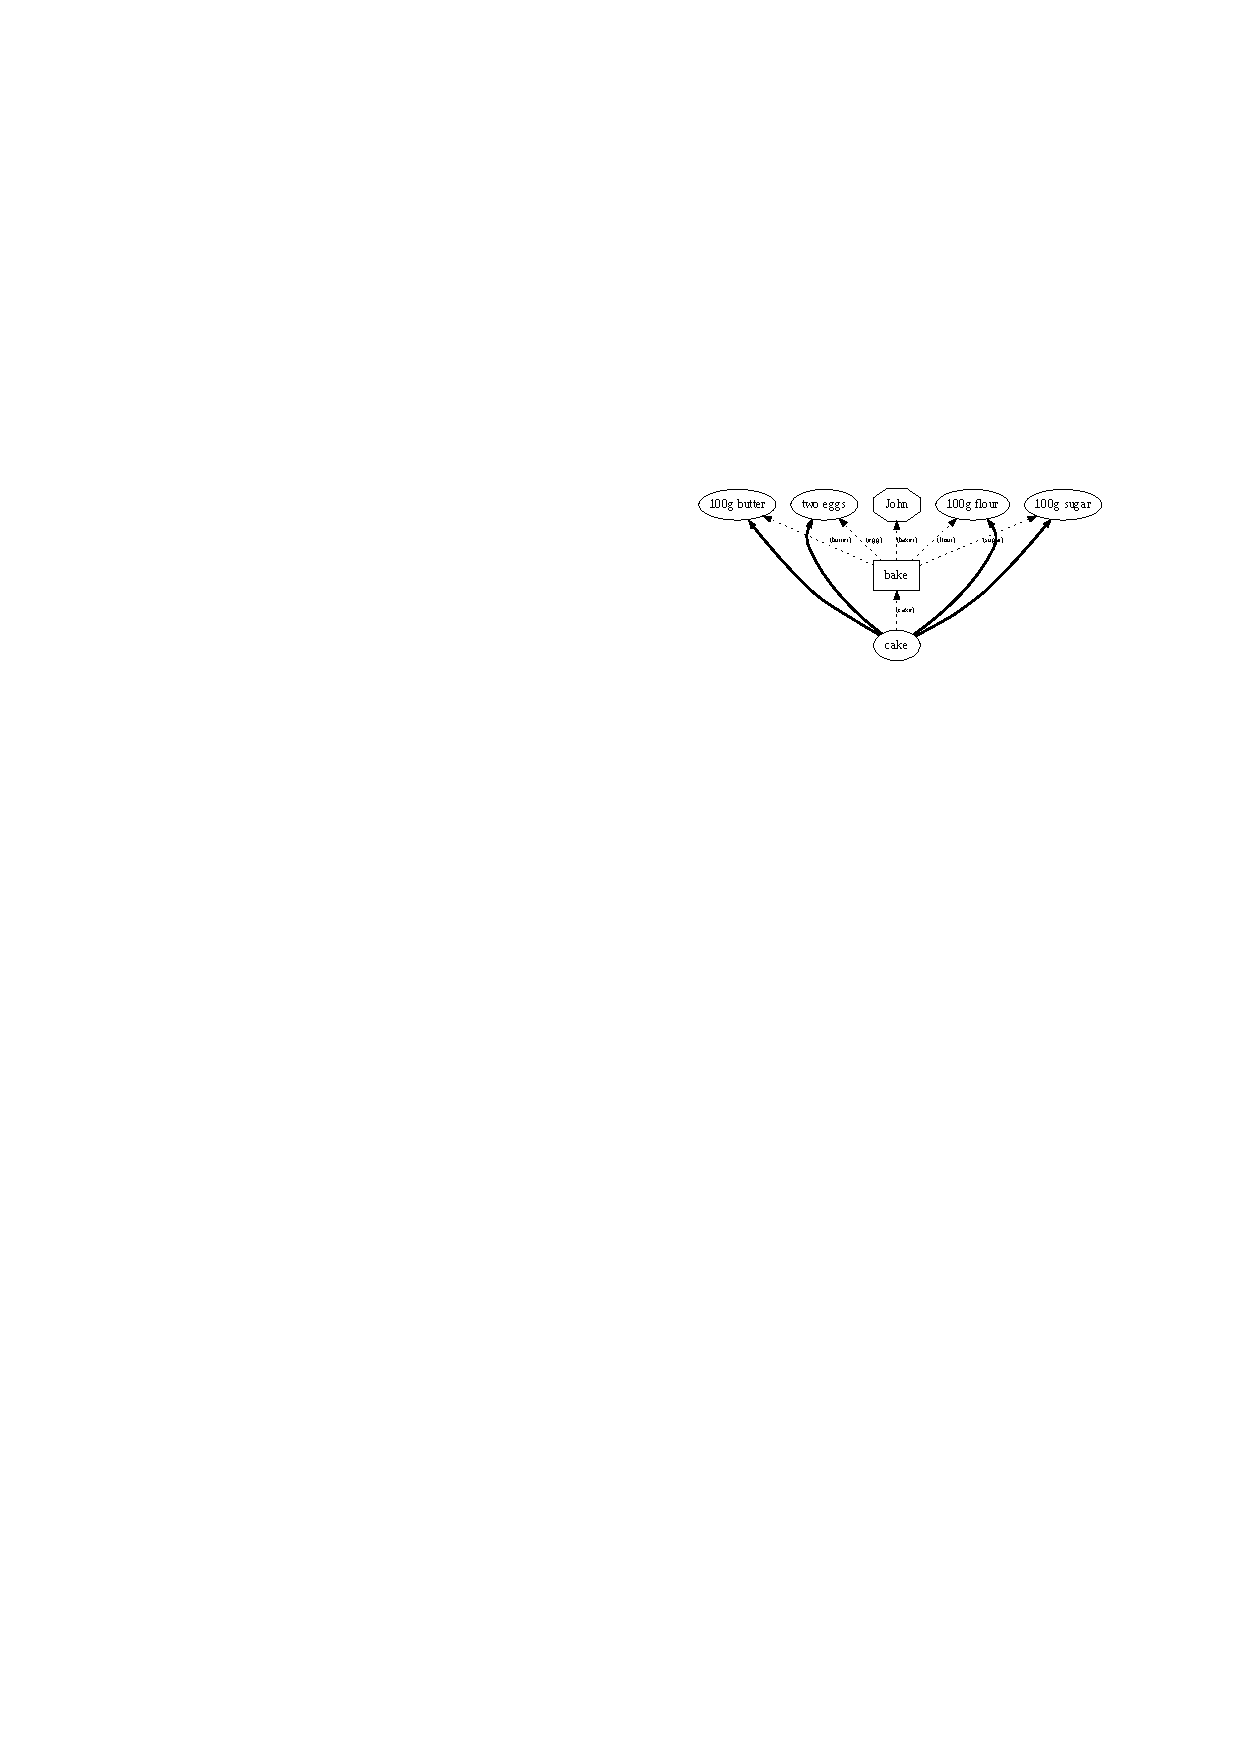
\includegraphics[width=\linewidth]{provenance-graph}
	\caption{A provenance graph for ``cake baking'' using the Open Provenance Model. The cake (artifact) was baked (the process) by John (the agent) using ingredients including butter, eggs, flour and sugar (artifacts). \is{Moreau2011}}
	\label{fig:lr-provenance-graph}
\end{figure}

The Open Provenance Model has been implemented in many systems, including notable scientific workflows such as Tarvena~\cite{Zhao2008}, Kepler~\cite{Bowers2006} and VisTrails~\cite{Bavoil2005}. The model is general and can be extended in both the structure and vocabulary to represent domain-specific problems. \emph{D-profile}~\cite{Groth2011} describes an extension of the model for representing provenance in distributed systems. ProveML~\cite{Walker2013} is another extension for recording the provenance of data, analytical process and interpretations in human terrain visual analytics.

\subsection{Analytic Provenance}
Analytic provenance focuses on understanding a user's reasoning process through the study of their interactions with a visualization~\cite{North2011}. It captures both the interactive data exploration process and the accompanied human reasoning process during sensemaking~\cite{Xu2015}. In this section, we discuss different models for representing analytic provenance data and methods to capture the data.

\subsubsection{Model}
Analytic provenance information can be categorized using a four-layer hierarchical model based on its semantic richness, proposed by Gotz and Zhou~\cite{Gotz2009}. \autoref{fig:lr-Gotz-Zhou-model} illustrates this model with the level of semantics increasing from bottom to top. The bottom-level \emph{events} consists of low-level user interactions such as mouse clicks and keystrokes, which have little semantic meaning. The next level up includes \emph{actions}, which are analytic steps such as querying the database or changing the zooming level of data visualization. The parameters such as data description and visualization settings are also part of the provenance. Further up are the \emph{sub-tasks}, which are the analyses required to achieve the sensemaking goal. Considering stock market analysis as the top-level \emph{task}, examples of sub-tasks could be identifying top performing companies and determining long term trends. 

\begin{figure}[!htb]
	\centering
	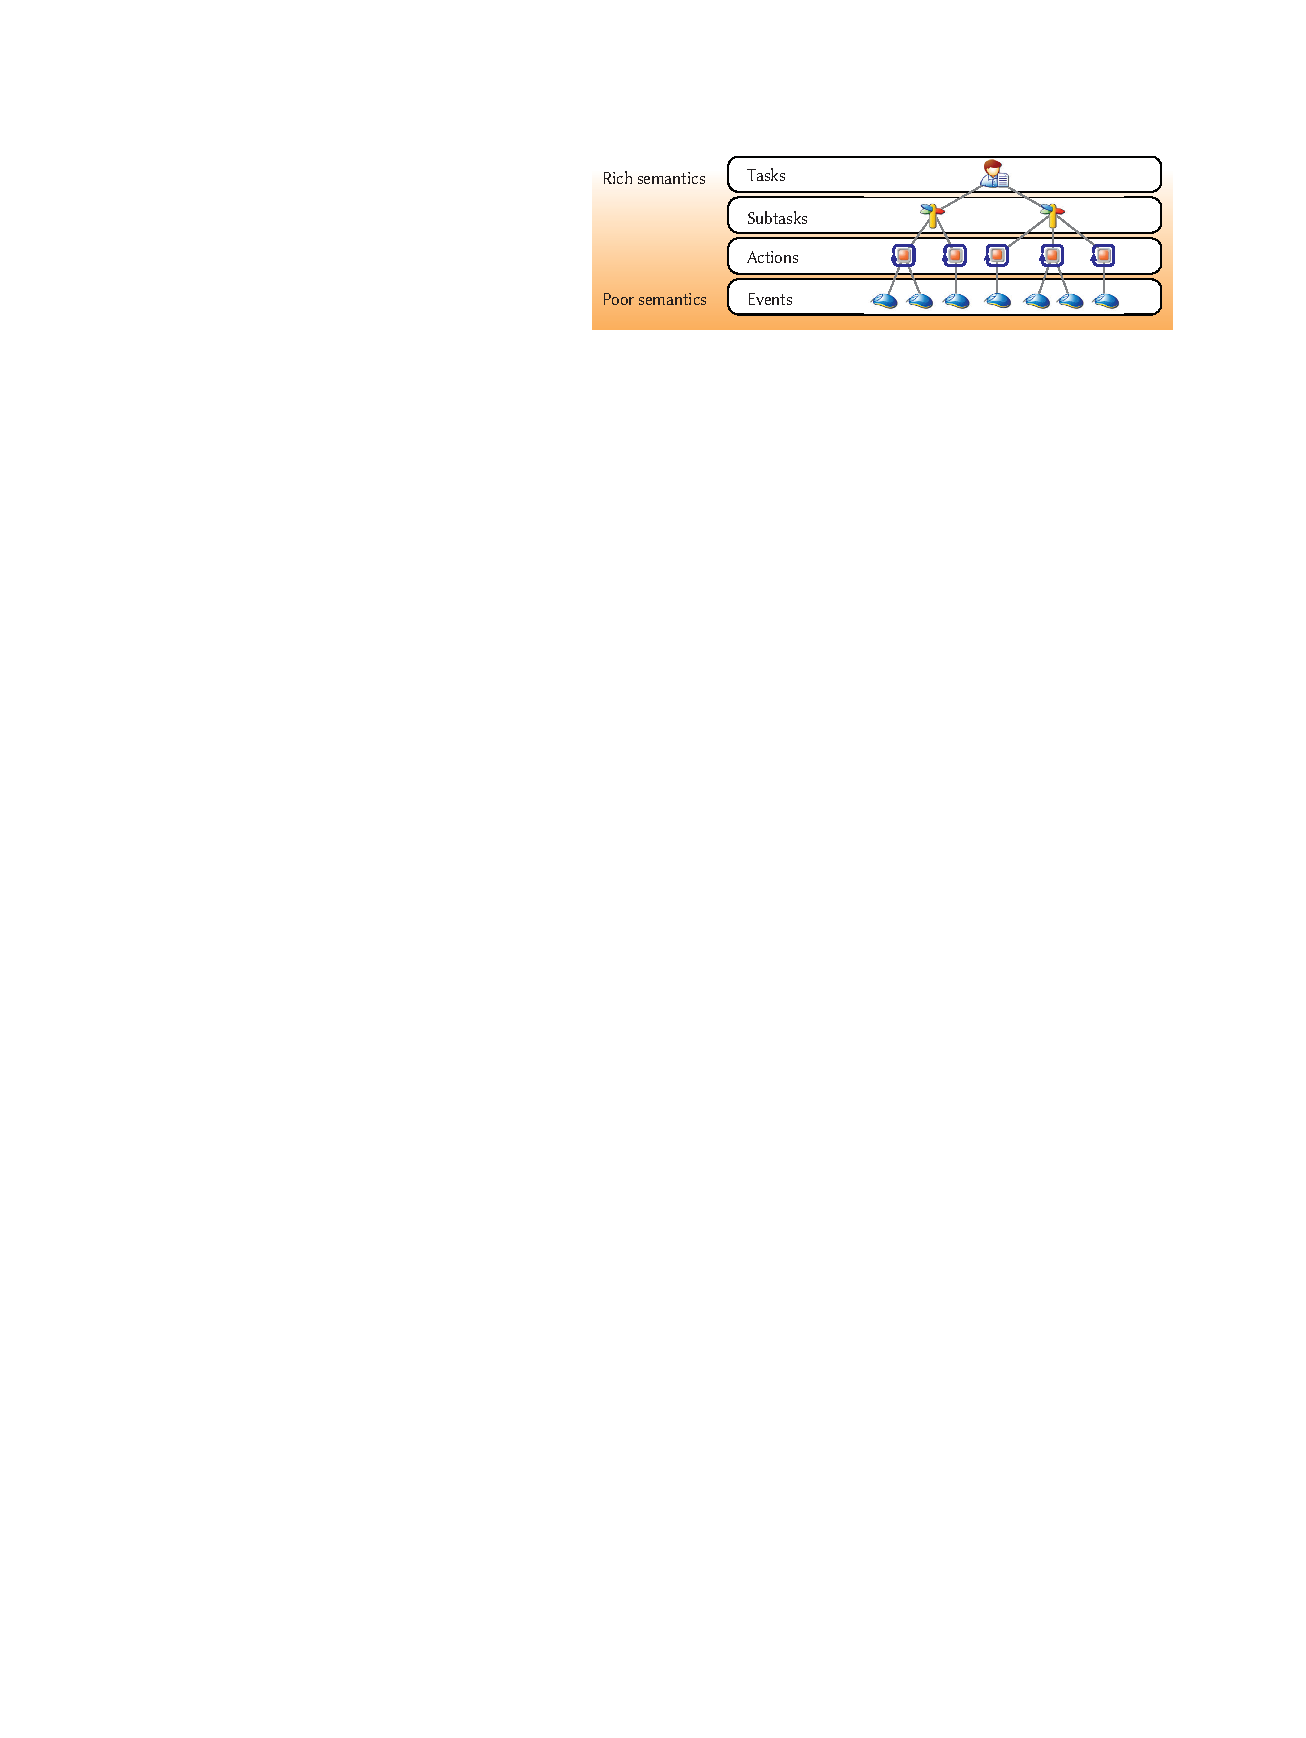
\includegraphics[width=.9\columnwidth]{Gotz-Zhou-model}
	\caption{The hierarchical analytic provenance model with semantic richness increasing from bottom to top. The bottom layer includes \emph{events} such as key presses and mouse clicks, which have little semantics. The next level up contains \emph{actions} such as the database query and visualization zooming. Further up level consists of \emph{sub-tasks}, which usually are the analyses performed during the sensemaking. The top level \emph{tasks} are the overall sensemaking undertaking. \is{Gotz2009}}
	\label{fig:lr-Gotz-Zhou-model}
\end{figure}

Analytic provenance is closely linked both within and across layers. Within a layer, analytic provenance is linked temporally (i.e., one event happens after another) and logically (e.g., one action depends on the two previous actions). A sequence of activities in each layer is performed to serve for a single activity in the next highest layer. For example, a database query action consists of several mouse click and key stroke events, and it is part of a higher level sub-task such as ``comparing stock performance''.

This four-layer model is general, allowing the designers to determine the specific activities they want to capture within each layer for their systems. For example, many existing taxonomies of visualization interaction and tasks can be used for the \emph{action} and \emph{sub-task} layers. Low-level analytic activities such as ``retrieve value'', ``sort'' and ``filter''~\cite{Amar2005, Gotz2009} can represent the \emph{action} layer. A taxonomy of interaction techniques based on their intent such as ``show me more related items'' may stay in-between the \emph{action} layer and \emph{sub-task} layer. A multi-level typology of abstract visualization tasks by Brehmer and Munzner~\cite{Brehmer2013} distinguishes why and how a task is performed, as well as what the task inputs and outputs are. The \emph{how} part of this typology is a good candidate for representing the \emph{action} layer, and the \emph{why} part may be suitable for the \emph{sub-task} layer.

A recent taxonomy by Ragan~et~al.~\cite{Ragan2016} characterizes provenance in visualization and analysis systems based on the type of provenance and the purpose of collecting it. Five ``flat'' provenance types include \emph{data}, \emph{visualization}, \emph{interaction}, \emph{insight} and \emph{rationale}. The type of data provenance is similar to what we describe previously in \autoref{sub:lr-data-provenane}. Visualization provenance concerns with the history of graphical views and visualization states, and interaction provenance focus on the history of user actions within a system. The combination of these two types of provenance is equivalent to the \emph{action} layer. Insight provenance describes the findings and rationale provenance explains the reasoning process that led to these findings. These two types of provenance are good candidates for the \emph{sub-task} layer.

\subsubsection{Capture}
Analytic provenance capture provides the data for its visualization. We describe capturing methods for each of the four layers in the Gotz and Zhou's model~\cite{Gotz2009}.

\paragraph{Events}
There is limited literature on capturing events because it is relatively easy and provides little semantics alone. Among these, Glass Box~\cite{Cowley2006} can record a wide range of low-level events such as mouse clicks, key strokes and window events. Its objective is to capture and archive intelligence analysis activities so they can be retrieved later. Simply capturing these events alone is insufficient to understand their purpose and rationale. For example, we know that a \textit{mouse click} is captured; however, what the purpose of that click was (e.g., to sort the data), and why the user performed that click (e.g., to find an interesting pattern from the data) are unknown. Commonly, when analyzing data with a visualization, an analyst needs to perform many operations with trials and errors to find the answer to the problem. In that case, a series of poor-semantic events makes it more difficult for the analyst to recall what has been done. Therefore, more meaningful activities also need to be captured. 

\paragraph{Actions}
During the course of analysis with a visualization, all user interactions can be systematically recorded. The visual exploration process can be modeled using a \textit{graph} metaphor. Nodes in the graph represent \textit{states} of the visualization and edges represent \textit{actions} that transform one state into another state. A state includes all the information required to reconstruct the captured visualization. For example, a state of a \textit{scatter plot} may include the dataset, attributes mapped to spatial positions, color and size. An action while interacting with a scatter plot could be changing attribute mapping of size. Commonly, \emph{undo/redo} features are provided to allow revisiting to previous states. If a new action is performed from a past state, a new branch will be created to store that new line of operations. 

Two common strategies can be applied to automatically capture the exploration process. The first strategy is to capture the initial state and all the actions so that they can be executed to reproduce any states~\cite{Kadivar2009}. This allows reapplying the analysis process with a different dataset, but could be time-inefficient if the number of actions is high. The second strategy is simply to capture all visualization states after each action~\cite{Bavoil2005}. This is easier to implement, but may be memory-expensive if a state contain too much information.

In the context of everyday, online sensemaking, users interact with a standard web browser instead of a visualization system. Visited web pages are automatically captured including visit time, web titles, URLs and favorite icons. Linking relationship between pages such as opening from a web link and using the browser's back button can also be captured~\cite{Ayers1995,Hightower1998,Milic-Frayling2003}. This results in a hierarchical history rather than a linear list of visited web pages in the standard history feature. Manual capture using bookmarks is also a standard feature of web browsers. It allows users to save web pages for revisitation purpose. Besides bookmarking a whole web page through its URL, a page element such as \textit{table} and \textit{form} HTML tags~\cite{Hong2008}, and a specific fragment of text~\cite{Dontcheva2006} can also be bookmarked. These finer-grained captures allow users to record what they want with higher accuracy. 

\paragraph{Sub-Tasks and Tasks}
Tasks and sub-tasks provide important clues to the purpose and rationale underlying the sensemaking. They describe an abstract summary of the task-solving process. However, they are largely part of users' thinking, which a visual analytics system does not have direct access to. Also, the time window to capture such information is very limited. Even the users themselves may forget what they were doing after a while, making it difficult to recover the analytic provenance information. Therefore, capturing high-level tasks and sub-tasks is one of the biggest challenges in analytic provenance capture.

Existing approaches to capture high-level analytic provenance can be broadly categorized into \emph{manual} and \emph{automatic} methods. The manual methods largely rely on users recording their analysis processes and sensemaking tasks, whereas the automatic methods try to infer the higher level tasks and sub-tasks from lower level events and actions. Even though the manual approaches are usually more accurate, they can distract users from the actual analysis tasks, which may discourage users from recording analytic provenance. Alternatively, the automatic approaches do not introduce interruption to the sensemaking process, but their capability of inferring semantic-rich analytic provenance information is limited~\cite{Gotz2009}. Individual differences also introduce additional challenges to designing a robust algorithm for the inferring process. Users' knowledge and experience have a considerable impact on the way they conduct analyses. As a result, the sensemaking process (i.e. the analytic provenance) can vary significantly from users to users, even with the same dataset and analysis task. 

\subparagraph{Manual}
User annotation is one of the most common forms in manual capture. Users create \emph{notes} or \emph{annotations} that are associated with certain data, analysis result, and/or visualization~\cite{Heer2009,Walker2013}. The content of a ``note'' is not limited to findings or discoveries; it can also include the thinking that leads to a finding or the relationships between findings. \emph{Data-aware annotation}~\cite{Heer2008a} links a finding and the associated visualization to the underlying data used to produce it, which makes it possible to apply new analysis and visual mapping at a later stage if further investigation is needed. 

Even though an individual note only represents a fraction of the analytic provenance, it is possible to provide a reasonably good overview of the sensemaking process if a number of notes and the connections between them are captured. For example, the \emph{Scalable Reasoning System} ~\cite{Pike2009a} allows users to record their discoveries of interesting patterns about the data, then specify their causal relationships, and generate a hypothesis based on these artifacts. However, this is only useful when users are willing to take notes, which can be perceived as distractions sometimes. Two common strategies to alleviate this include minimizing interruption/cognitive effort~\cite{Hong2008} and providing immediate benefits to the sensemaking task such as planing exploratory analysis for complex tasks~\cite{Lunzer2014}. However, currently there is a lack of general design guidelines for how to achieve them, and there are few user studies evaluating how effective they are, in terms of both the benefits they bring and the potential cognitive cost they can introduce. 

\subparagraph{Automatic}
One of the main disadvantages of manual capture is the requirement of direct input from users. Automatic approaches try to address this by inferring higher level analytic provenance from what can be automatically captured. As discussed earlier, it is easier to capture analytic provenance at the event and action level. Therefore, most automatic approaches try to infer sub-task and task-level information from event and action provenance.

This turns out to be a difficult challenge. An experiment studied how much of a user's reasoning process can be recovered from user action information~\cite{Dou2009}. A domain-specific sensemaking task was used and experts were recruited to analyze the user action log. Higher-level analytic provenance manually inferred from the interaction logs were compared with the ground truth obtained through interview. The results showed that 79 percent of the findings, 60 percent of the methods, and 60 percent of the strategies were correctly recovered. The accuracy is not high even in such a constrained setting with domain experts doing the inference. Given the diversity of data and analysis involved in the sensemaking and the difficult of replicating expert knowledge/thinking in a computer system, the chance of having a generic technique that can accurately infer semantic-rich analytic provenance information for a variety of analysis tasks is not high.

Instead, existing methods either constrain the problem/analysis domain or aim for less semantically rich analytic provenance. By limiting the choice of data and analysis/visualization, an inference algorithm has better chance to make the right guess. However, even within a specific domain (such as finance), the types of data and analyses involved are still of very large amount. Also, being limiting on the data and analysis can constrain the system capability, having a negative impact on the sensemaking task.

Given the difficulty of inferring task/sub-task information, a few methods target less semantic-rich provenance. One such example is \emph{action chunking}, i.e., identify a group of actions that are likely to part of the same sub-task, without knowing what the sub-task is. Such approaches apply heuristics to infer patterns from action logs based on repeated occurrence and proximity in data/visualization space or analysis time~\cite{Gotz2009}. Such chunking information can be useful in several ways. For example, the system can prompt user to take a note if such an action usually occurs within a specific sequence. Also, the grouping information can be used for aggregation when large amount of provenance information is to be visualized. This method is later extended to monitor user behavior for implicit signals of user intent and uses the information to suggests alternative visualization~\cite{Gotz2009}. It is an open research problem to explore similar analytic provenance that can be effectively inferred and provides semantic information that can be used for supporting sensemaking.